\documentclass{article}

\usepackage{amsmath}
\usepackage{graphicx}
\usepackage{listings}
\usepackage{color}


\usepackage{xepersian}
\settextfont{BNazanin} 
\linespread{1.3}
\newcommand{\linia}{\rule{\linewidth}{0.5pt}}

\def\LOGO{
\begin{picture}(0,0)\unitlength=1cm
\put (0.5,0) {
\includegraphics[width=5.1em]{fanni.jpg}}
\end{picture}
}

\def\LOG{
\begin{picture}(0,0)\unitlength=0.5cm
\put (-6,0) {
\includegraphics[width=4em]{logo.png}}
\end{picture}
}

\definecolor{mygreen}{rgb}{0,0.6,0}
\definecolor{mygray}{rgb}{0.5,0.5,0.5}
\definecolor{mymauve}{rgb}{0.58,0,0.82}

\lstset{ 
  backgroundcolor=\color{white},   % choose the background color
  basicstyle=\footnotesize,        % size of fonts used for the code
  breaklines=true,                 % automatic line breaking only at whitespace
  captionpos=b,                    % sets the caption-position to bottom
  commentstyle=\color{mygreen},    % comment style
  keywordstyle=\color{blue},       % keyword style
  stringstyle=\color{mymauve},     % string literal style
}


\begin{document}

\title{\LOG به نام خداوند بخشنده مهربان \LOGO }
\author{ تمرین شماره ۲\\ نازنین صبری}
\date{۱۵ اسفند ۱۳۹۶}
\maketitle

\renewcommand{\labelenumii}{\alph{enumii}}
\textbf {در تمامی سوالات هدف الگوریتمی با زمان اجرای بهینه است و در صورت بهینه نبودن بخشی از نمره از شما کسر خواهد شد}
\begin{enumerate}
	\item  تبدیل‌های خواسته شده را انجام دهید.\\ 
	\begin{enumerate}
 		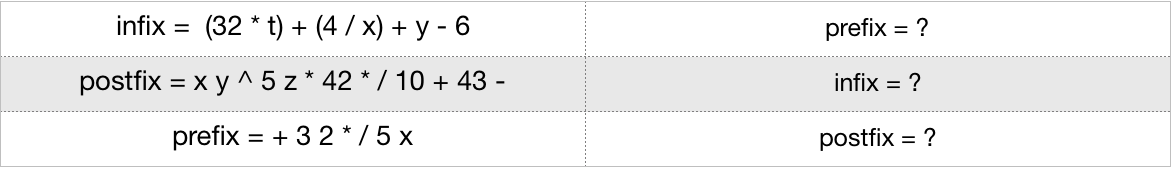
\includegraphics[scale=0.6]{./Q1}
	\end{enumerate}
	\item الگوریتمی بنویسید که درست بودن پرانتز‌ها، کروشه‌ها و ... باز و بسته را تشخیص دهد، ورودی این تابع یک عبارت است. به عنوان مثال اگر ورودی \lr{1 + {(1+[2*3])}} باشد تابع باید بررسی کند که به ازای هر پرانتز باز علامت بسته‌ی آن نیز در جای مناسب وجود دارد و به همین صورت برای سایر علامت‌های باز و بسته و در نهایت برای این ورودی خاص باید اعلام کند که درست است، در صورتی که اگر ورودی \lr{ 1+{(1+[2*)3]}} باشد باید اعلام کند که عبارت داده شده نادرست است. 
	\item 
	\begin{enumerate}
		\item)  توضیح دهید که چگونه می‌توان ۲ \lr{Stack} را به کمک یک آرایه نمایش داد. نشان دهید که عمل \lr{push()} و \lr{pop()} در روش شما چگونه انجام خواهند شد. 
		\item)  توضیح دهید که چگونه می‌توان \lr{n} تا \lr{Stack} را به کمک یک آرایه نمایش داد، مشابه بخش قبل روش انجام \lr{push()} و \lr{pop()} را بیان کنید. 
	\end{enumerate}
	\item الگوریتمی بنویسید که مقدار عددی عبارت \lr{postfix} داده شده به آن را محاسبه کند. به عنوان مثال اگر عبارت داده شده به الگوریتم \lr{30 3 5 * / 1 + 10 +} باشد الگوریتم باید عدد ۱۳ را به عنوان خروجی بدهد. 
	\item با استفاده از \lr{Stack} الگوریتمی بنویسید که آرایه‌ی \lr{A} را به عنوان ورودی بگیرد و آرایه‌ی خروجی را به این صورت بسازد که عنصر \lr{i} ام آن اولین عدد بزرگ‌تر از عنصر \lr{i} ام آرایه \lr{A} ، در آن آرایه است. به عنوان مثال اگر آرایه ورودی \lr{[12, 3, 1, 2, 7, 25]} باشد، خروجی الگوریتم به صورت \lr{[25, 7, 2, 7, 25, -1]} خواهد بود. در خروجی برای آخرین عنصر در آرایه ورودی -۱ را چاپ می‌کنیم. 
	\item آرایه‌ای نامرتب و عددی داریم. شبه کدی بنویسید که مشخص کند که آیا در آرایه داده شده ۲ عنصری وجود دارند که حاصل جمع آن‌ها با عدد داده شده برابر باشند. به عنوان مثال اگر آرایه ما \lr{[1, 4, 2]} باشد و عدد مورد نظر \lr{x = 3} باشد خروجی بله است چون حاصل جمع ۱ و ۲ برابر با ۳ می‌شود. 
	\item الگوریتمی بنویسید که محتوای یک \lr{Stack} را با کمک گرفتن از یک \lr{Stack} کمکی \lr{sort} می‌کند. 
\end{enumerate}

\newpage


\end{document}